%
% $Id: ch01_overview
%
%   *******************************************************************
%   * SEE THE MAIN FILE "AllegThesis.tex" FOR MORE INFORMATION.       *
%   *******************************************************************

\chapter{Introduction}\label{ch:intro} % we can refer to chapter by the label

%   ************************************************************************
%   * In LaTeX, new paragraphs are begun by simply leaving a blank line in *
%   * the LaTeX file.                                                      *
%   *                                                                      *
%   * The \\ characters should NEVER be used to end a paragraph.           *
%   * They are used only for inserting line breaks in certain situations.  *
%   *                                                                      *
%   * "Widows" (ending paragraph lines at the top of a new page) and       *
%   * "orphans" (opening paragraph lines at the bottom of a page) should   *
%   * be eliminated; this sometimes requires re-writing some of the        *
%   * text to change the line lengths.                                     *
%   ************************************************************************

Our research focuses on the development and comparison of intelligent agents for playing perfect information games.  Specifically, we implement agents for playing the games Go and Hex, which we will thoroughly describe later.  The agents each include modifications to the Monte-Carlo Tree Search algorithm which have been previously implemented or proposed by researchers.  Each modification of Monte-Carlo Tree Search has been empirically proven to improve upon various applications of the algorithm, but have not been directly compared to one another in the same environment.  We provide a direct comparison between the agents by comparing their performance in several variations of Go and Hex.

The purpose of this chapter is to outline our motivation behind researching this problem, further state the goals of our research, and introduce the Monte-Carlo Tree Search (MCTS) algorithm, which is very widely used for game-playing agents.  We also explain the rules of Go and Hex, as well as some common structures found within the games which we utilize in one of our agents.  Lastly, we provide an overview of the structure of this paper.

\section{Motivation} \label{sec:motivation}
A major long-term goal of artificial intelligence research is to create a general intelligent agent --- a machine which can act independently, and intelligently, in a variety of situations.  In other words, create a machine which is able to mimic a human's intelligence.  Specifically over the last decade, researchers have become increasingly close to achieving this goal; for some tasks, AI systems are able to match or even exceed a human's performance.  For example, in recent years, research into deep neural networks has led to systems which perform very well at pattern recognition problems \cite{imagenet}.  Using a large amount of training data, they are able to label objects in images \cite{imagenet}, interpret human speech \cite{HintonDeng}, distinguish faces from one another \cite{parkhi15}, and even mimic human speech \cite{wavenet}.  Essentially, such systems can learn to mimic human senses and classification abilities.

While this is certainly impressive, human intelligence is defined by far more than recognizing patterns and understanding the things we sense.  The ability to react to our world, make decisions on the fly, and adapt to changes is a better measure of human intelligence.  Essentially, our decision-making abilities are not limited to a finite set of problems --- regardless of the task, we are able to work towards finding a solution.  Thus in order to progress towards the goal of a more generalized AI, we need to work on building systems which can exist, adapt, and function in changing environments.

One's first instinct in developing a general AI may be to use physical robots as intelligent agents and the real world as an environment.  Robots have been (and continue to be) used in AI research and competitions --- for example, the RoboCup Soccer \cite{robocup} tournament is an annual competition which pits cooperative multi-agent robot systems against one another in games of soccer (Figure \ref{fig:robocup}).  The teams of robots consistently improve every year.  Despite this, their limitations are very obvious.  At RoboCup, there are several examples of robots failing to do what they were designed to, sometimes in spectacular fashion.

\begin{figure}[h]
    \centering
    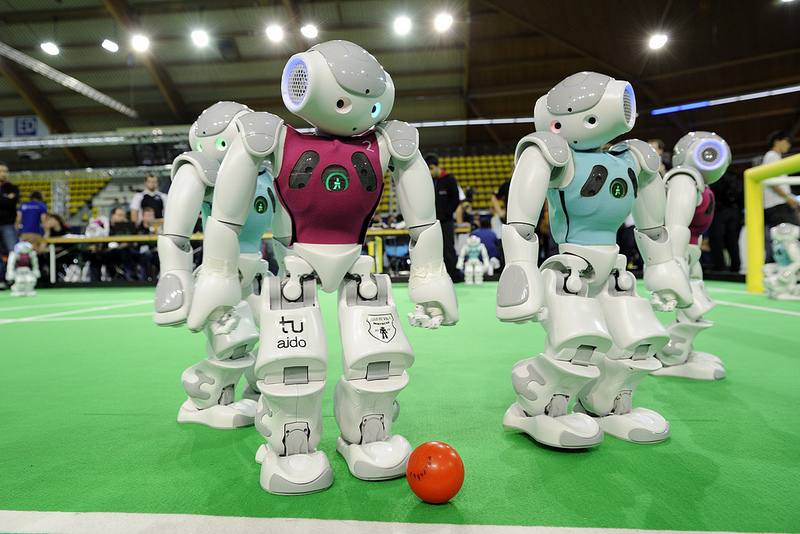
\includegraphics[clip, scale=.25]{images/robocup2015.jpg}
    \caption{RoboCup 2015 \cite{robocup}}
    \label{fig:robocup}
\end{figure}

Robots are simply not an ideal way to develop artificial intelligence --- robots are expensive to build, time-consuming to test, and their effectiveness is bottlenecked by their physical limitations \cite{Gunderson, Bihlmaier}; they are not an effective way to test new algorithms.  Furthermore, there are many variables of the real world which we are simply unable to control effectively, e.g. gravity.  Robots do hold a very important place in the field of AI and computer science in general, but they are not suited for testing new and improving algorithms.  On the other hand, purely virtual environments --- specifically computer board games --- are perfect for experimentation for several reasons.

When working with pure software agents rather than robots, we do not need to worry about the physical efficacy and limitations of the agents --- the integration of hardware and software is not needed.  Meanwhile, a board game has a set of rules which cannot be broken, and a very obvious goal for everyone in the game: to win.  Furthermore, the rules and win-conditions can be tweaked as needed, and the game can be sped up to allow for quick learning and testing.  Simply put, such games offer extremely controllable environments.  The clear goal (to win) allows for very easy experimentation and testing of game playing agents.  To see how an agent compares against humans, we can simply have the agent play a number of humans to see how often it wins.  We can also have two different agents compete head to head against one another in order to compare two different algorithms.

Perfect information games are a subset of games for which each player has access to all of the game information --- nothing is hidden from either player.  For example, chess and go are both perfect information board games as both players know the location of any and all pieces on the board.  However most card games, or a game such as Stratego, are imperfect information as the value of each players pieces are hidden from one another \cite{Policonomics}.

When comparing two agents in a head to head game, we consider perfect information to be superior to imperfect information games.  This is because perfect information ensures that the reason for an agent's win is actually a superior algorithm.  In an imperfect information game, there could be pieces of information which are more valuable than other pieces of information --- results of the game could be skewed towards whichever AI stumbles upon this information first \cite{Gilpin}.  For example, in Stratego, the value of a player's piece is hidden from their opponent until an "attack" is made against the piece --- if one player happens to find higher level pieces than their opponent early in the game, the game may become skewed in their favor through pure luck.  While it may be possible to account for such situations (or perhaps such imbalances may begin to even out over many trials), it can be easier to just begin with a perfect information game.

For any game, we can think of the ``state'' of the game at any time to be a snapshot of the game at that moment, or rather a recording of all of the game's information at that specific time.  For turn-based games, the current game game state changes exactly when a player makes a move during his/her turn.  In any intelligent game-playing agent, the most important factor is the ability of the agent to evaluate the game state --- that is, the methodology it uses to determine the probability of winning the game for a given state.  For this, one might consider building a system which attempts to identify patterns among positive game states and construct a set of beliefs to approximate the value of any given state; this set of beliefs can be thought of as a heuristic or evaluation function.  However, building an adequate evaluation function for a game state is a very complex task; in fact, there has been much research into using heuristic analysis for games with little success \cite{chaslot2008monte}.

Tree search methods are another way of determining the value of a game state.  A tree search method simulates a number of games from the given state, attempting to fully construct a tree of all possible game configurations from the current state.  Each game state can be represented as a node in a tree, with a move which results in moving from one state to another being represented by a link between nodes  --- this tree representation of a game is called a game tree.  We loosely refer to the rate at which each level of the game tree increases in size as the branching factor of the game.  Rather than trying to directly analyze the value of a given game state, a tree search method determines value of a game state by finding how many paths to a winning position exist.

As a tree search algorithm runs, the game tree becomes fuller; once the tree is full, an agent utilizing it is able to play perfectly --- that is it will always win provided it is possible.  The downside of many tree search algorithms is that they are not useful until the game tree is at least mostly full.  In the minimax algorithm, for example, a node's value cannot be determined until the value of every one of its children down to the leaf nodes is found \cite{minimax}.  For a game such as Go, this is impossible to achieve in any reasonable amount of time --- a single game of traditional 19x19 Go has over $2 \times 10^{170}$ possible playouts.  The exact number of possible Go games was only recently calculated, and required an estimated 30 petabytes of disk I/O \cite{Trompfinal}.  Due to the sheer amount of storage which would be needed to track each possible game state, it would be impossible to even come close to actually constructing the whole game tree.

Over the last decade, game AI development has moved away from basic tree search and towards methods involving the Monte-Carlo Tree Search (MCTS) algorithm \cite{browne2012survey}.  MCTS asymmetrically explores the game tree by taking into account both the current estimated value of each child node, and the number of times each child node has been visited in a simulation.  The specific method of exploration can be customized by considering one of these factors more heavily than the other.  MCTS is also different from other tree search algorithms as it does not need to construct an entire game tree in order to make a decision.  Such methods have proven far more successful, as MCTS-based AIs have since become some of the most successful game AIs in the world \cite{alphago}\cite{benzene}.
%   *******************************************************************
%   * FIGURES ARE PLACED ACCORDING TO A SET OF CONSTRAINTS THAT CAN   *
%   * BE MANIPULATED TO SOME DEGREE.                                  *
%   * A SEARCH FOR "controlling latex floats" TURNS UP A NUMBER OF    *
%   * SITES THAT HAVE USEFUL INFORMATION, FOR EXAMPLE:                *
%   *                                                                 *
%   * http://mintaka.sdsu.edu/GF/bibliog/latex/floats.html            *
%   * http://goo.gl/aC8E8Q                                            *
%   * http://robjhyndman.com/hyndsight/latex-floats/                  *
%   *******************************************************************

\section{Monte-Carlo Tree Search}\label{sec:mcts}
Monte-Carlo Tree Search (MCTS) is a selective search method for finding optimal decisions via random sampling. Since its development in 2006, it has been widely used for the creation of game AI, specifically for games which can be represented as a finite tree of moves \cite{chaslot2008monte, browne2012survey}.  Prior to its development, the minimax algorithm was commonly used as the basis for finite-game playing agents.  An explanation of the minimax algorithm is outside the scope of this paper, but an in-depth explanation of the algorithm can be found in \cite{minimax}.

MCTS is superior to previous tree search methods such as minimax for a couple of reasons.  First, while an agent utilizing minimax guarantees optimal play, minimax requires the entire game tree be explored --- this often requires an impractical amount of time for games with even just a moderate branching factor.  MCTS, however, can be interrupted at any time and return a node to explore.  Second, given adequate time, MCTS provides optimal play given adequate memory and time --- in fact, MCTS converges to minimax \cite{browne2012survey}.  So essentially, MCTS can provide accurate decision making without the potentially exponential time complexity of minimax.  

MCTS works in four steps as depicted in Figure 2: Selection; Expansion; Simulation; and Backpropogation.
\begin{enumerate}
    \item  Selection: Starting at the root of the tree, child nodes are selected recursively until a leaf node $L$ is reached.  The way in which these children nodes are selected is called the \textit{tree policy}, and is discussed below.
    
    \item Expansion: if $L$ is not a terminal node for the game tree, a child node $C$ is created.  Depending on the application of MCTS, more than one child node may be chosen.
    
    \item Simulation: Simulate a full play of the game from node $C$.  In the simulation step, the tree policy is not used during the simulation.  Rather, a \textit{default policy} is used --- most commonly, the default policy is a simple random selection from possible moves until a terminal condition is met.  Note that the nodes visited during simulation are not added to the tree.
    
    \item Backpropogation: The tree is updated with the results of the simulation.  Specifically, each node's estimated value is updated (based on the outcome of the simulation), as well as the number of times it has been visited.
\end{enumerate}

\begin{figure}[h]
    \centering
    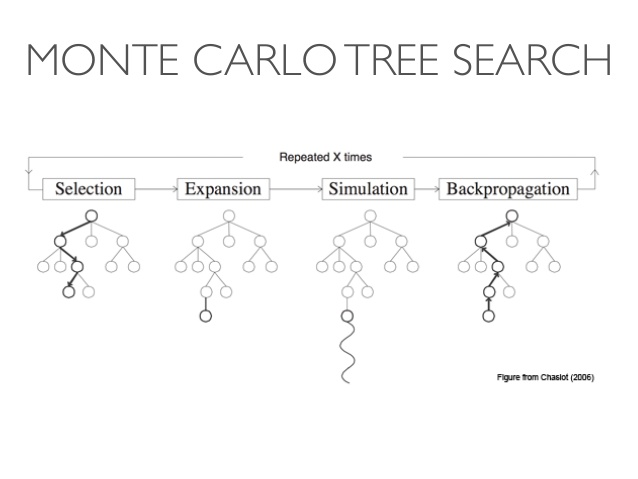
\includegraphics[clip, trim={0 4cm 0 5cm}, scale=.6]{images/mcts.jpg}
    \caption{Monte-Carlo Tree Search algorithm \cite{chaslot2008monte}}
    \label{fig:MCTS}
\end{figure}

During the selection phase, there is a trade-off between \textit{exploitation} and \textit{exploration} --- should we \textit{exploit} the nodes whose rewards we already know, and continue to expand a well searched path, or should we \textit{explore} the less visited nodes in hopes of finding a better option \cite{nakhost2009monte}?  A widely used tree policy to balance these options is called Upper Confidence Bounds for Trees (UCT).  When using UCT as the tree policy, a child node which maximizes the following is chosen:
    
\begin{equation}\label{eq:UCT}
    UCT = v_i + C * \sqrt{\frac{2\ln N}{n_i}}
\end{equation}
    
where $v_i$ is the estimated value of the node, $n_i$ is the number of the times the node has been visited and $N$ is the total number of times that its parent has been visited.  $C$ is a constant bias parameter which we can change as we wish.  In this formula, $v_i$ represents exploitation, while the rest of the equation represents exploration.  So, by properly tuning the value of $C$, we are able to find a balance between exploitation and exploration \cite{lucas2014fast}\cite{audibert2009exploration}.

While MCTS can be rather effective in its most basic form, it is further enhanced using a variety of machine learning techniques.  Most of the industry leading game-playing agents utilize an MCTS decision making algorithm with the integration of some other AI techniques --- most often, some form of Artificial Neural Network (ANN) or Genetic Algorithm (GA) is used \cite{browne2012survey}.  These algorithms and existing implementations of game-playing agents which utilize these algorithms will be discussed in Chapter 2.

%It is the privilege of the thesis author (in consultation with the
%project supervisor and other readers) to decide on the best way to 
%organize the sections and chapters in the way that makes the most sense.
%If the introduction begins with a motivating
%anecdote, perhaps this is best followed by defining a few terms or mentioning
%some major results that the reader should be aware of right from the 
%beginning. But 

\section{Games}\label{sec:games}
In this section, we outline the perfect information games we use for our experiments: Go and Hex.  Due to their high branching factor, Go and Hex are two rather well-known and well-studied games in the field of AI.  The purpose of this section is to give the reader an understanding of the basic rules, and overview a few common structures within the two games in order to provide a deeper understanding of strategy.

\subsection{Go}
Go is a two-player game usually played on a 19x19 board, although any size board can be used and boards of size 9x9, 13x13, and 17x17 are particularly common.  The rules of Go are very simple.  The players take turns placing stones on the board, attempting to surround more territory than the other player.  Stones cannot be removed, but if one or more of a player's stones are completely surrounded by the other's, the surrounded stones are removed from the board (Figure \ref{ref:gogui}).  The game continues until either neither player wishes to move one player resigns, or there are no legal moves remaining on the board.

\begin{figure}[h]
\centering
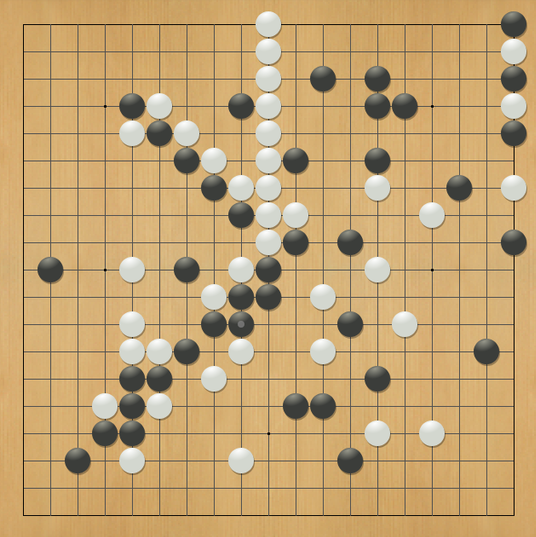
\includegraphics[scale=0.25]{images/gogui.png}
\caption{An example of a Go board generated in GoGui \cite{fuego}}
\label{ref:gogui}
\end{figure}

Despite its simple rules, Go has over $2 \times 10^{170}$ possible playouts, making it one of the most computationally complex board games ever created \cite{Trompfinal}.  The combination of this fact with its popularity as a game has led to it being the focus of a large amount of research compared to other games.

Go has many well-defined board structures, but some of the most common and important concepts are that of \textit{liberties}, \textit{atari}, and \textit{seki}.  Each stone has between zero and four liberties, a liberty being an open space directly adjacent to the stone.  For example, a stone which is placed such that it is not touching any other stones is said to have 4 liberties.  A region of stones is said to be in atari if the entire region has only a one liberty --- that is, if the entire region could be captured in a single move by the other player.  Seki refers to empty spaces which cannot be safely played on by either player --- a space is in seki if placing a stone on the space would immediately allow the other player to capture a region.  In figure \ref{fig:seki}, the two spaces marked in green are in seki because if a player were to place a stone in one of them, the other player would be able to immediately surround and capture a region by placing a stone in the other.

\begin{figure}[h]
\centering
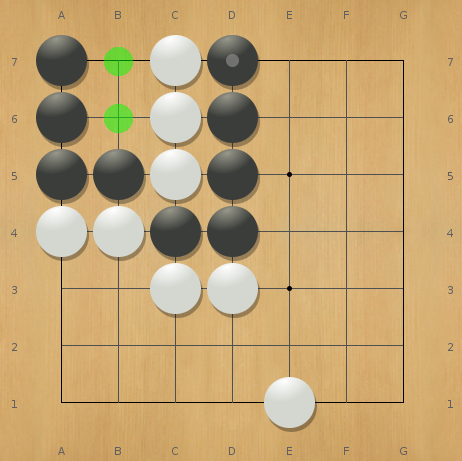
\includegraphics[scale=0.35]{images/seki.png}
\caption{Example of seki in Go}
\label{fig:seki}
\end{figure}

There are various methods of scoring a game of Go.  The simplest of these is the \textit{stone scoring} method, which was popular in the past but is usually no longer used \cite{goscore}.  Under this scoring method, each player's score is determined by how many of his pieces are on the board; the player with the most pieces on the board at the end of the game is the winner.  This method of scoring has given way to the \textit{territory scoring} method \cite{goscore}.  Under territory scoring, a player's score is determined as:
\begin{itemize}
\item The number of empty spaces on the board which which only the player's stones surround,
\item minus the number of empty spaces on the board which are surrounded and in seki,
\item minus the number number of the player's stones which have been captured;
\item minus the number of ``dead'' stones, i.e. stones which both players agree would be captured by the end of the game.
\end{itemize}

The last aspect of territory scoring makes it very hard to determine territory score programmatically.  Players can argue that any of their pieces on the board are not dead even if their removal is seemingly inevitable.  At the same time, both players can agree to certain pieces being dead even if they appear to be far from being captured; territory scoring has a decidedly human element to it.

\subsection{Hex}
Hex is a two-player board game usually played on a hexagonal grid, usually a 14x14 rhombus as shown in Figure \ref{ref:hex}.  Each player takes turns placing a stone on a cell of the grid, and simply attempts to link their two opposing sides before the opponent links the other two.  The first player to connect their two sides wins.  The only other rule is that, due to the first player to move having a distinct advantage, the second player can choose to switch positions with the first player after the first move.

\begin{figure}[h]
\centering
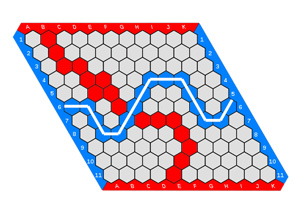
\includegraphics[scale=0.4]{images/hex.jpg}
\caption{A winning game for blue \cite{hexwiki}}
\label{ref:hex}
\end{figure}

A game of Hex has a branching factor similar to that of a game of Go on the same size board, but Hex games are usually far shorter, and also much less computationally expensive to simulate \cite{goscore}.  This is because of a simpler, better-defined end game condition (a connection between opposite sides), as well as the fact that pieces never have to be removed from the board.  Games can end with the majority of the board being empty, and we never need to check if a piece should be removed from the board as we do in Go.  One interesting aspect of Hex which differs from Go is that Hex cannot end in a draw; if every space on the board is filled, there must exist a path between two opposite edges \cite{goscore}.

\begin{figure}[h]
\centering
\begin{minipage}{.5\textwidth}
  \centering
  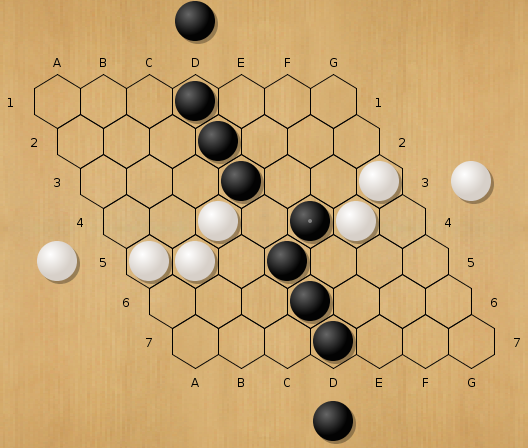
\includegraphics[scale=0.3]{images/hexbridge.png}
  \captionof{figure}{A bridge structure in Hex}
  \label{fig:hexstruct2}
\end{minipage}%
\begin{minipage}{.5\textwidth}
  \centering
  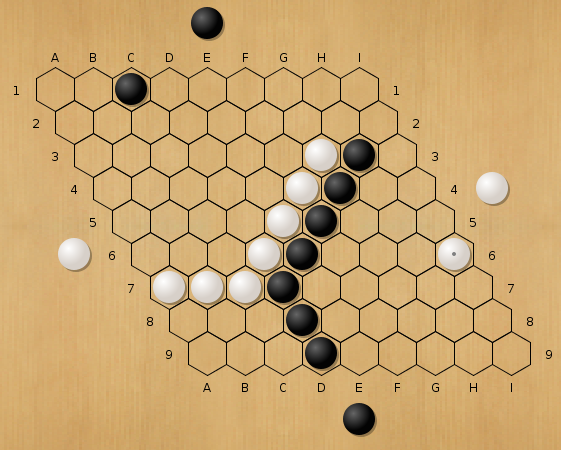
\includegraphics[scale=0.3]{images/hexladder.png}
  \captionof{figure}{A ladder structure in Hex}
  \label{fig:hexstruct1}
\end{minipage}
\end{figure}

Hex has far fewer well-defined board structures than Go.  In fact, it only has two: \textit{bridges} and \textit{ladders}.  A bridge refers to a structure wherein two seperate regions of a players pieces will be able to be connected in one move, regardless of where the opponent plays.  A ladder refers to a structure where a string of one players stones is placed immediately.  Figure \ref{fig:hexstruct1} provides an example of a bridge for black, and \ref{fig:hexstruct2} provides an illustration of a ladder being formed.

\section{Goals of the Project}\label{sec:goals}
As stated previously, most of the current top-performing game-playing agents utilize MCTS with some integration of a machine learning algorithm.  These agents are almost always shown to perform better than agents using just MCTS or other decision making algorithms.  However, they have rarely if ever been directly compared to one another.  This thesis helps fill this gap in research.  We implement a number of intelligent game-playing agents using MCTS integrated with machine learning algorithms which have been utilized in current, leading systems. These agents are benchmarked against one another on the perfect information games Go and Hex.  This provides a concrete, direct comparison of existing techniques, and a clear heirarchy between these techniques is shown.

The use of multiple games is important in these tests.  While the performance of standard MCTS is game-independent, the performance of heuristic techniques is often quite dependent on the game, as stated earlier.  When we integrate MCTS with these different AI algorithms, we are essentially introducing a small heuristic bias in the way MCTS performs.  Using multiple games helps show how this introduction of a heuristic bias affects how game-dependent the performance of the agent is.

% COMMENTED OUT NEXT FEW LINES TO SAVE SPACE; MAY PUT THEM BACK LATER
%Following the concise statement of the thesis, some of the details can be
%expanded.  
%It is appropriate to
%refer to some of the results in the introduction (which may 
%mean going back and adding them to the introduction once the
%research is completed). 
%A senior thesis, or any research paper, is not a mystery 
%novel---there is no need to keep the reader in suspense about what
%has been accomplished.

\section{Thesis Outline}\label{sec:outline}
Chapter two introduces the different AI algorithms we integrate into MCTS, and also describes existing implementations utilizing these algorithms.  Each section of the chapter focuses on a different algorithm, and outlines a game-playing agent which has been implemented using such an algorithm.  The chapter also discusses the Encog machine learning library which we use extensively in our implementation.  Chapter three goes over the structure of our game-playing framework, the implementation of the different games and agents, and our experiment design.  Chapter four contains the results of our experiments, and we briefly explain any trends in the data.  Finally, we provide an analysis of our results and discuss any future research or improvements which could be made to the code base in Chapter five.